\documentclass[a4paper, 10pt]{article}
\usepackage[utf8]{inputenc}
\usepackage{verbatim}
\usepackage{listings}
\usepackage{graphicx}
\usepackage{a4wide}
\usepackage{color}
\usepackage{amsmath}
\usepackage{amssymb}
\usepackage[dvips]{epsfig}
\usepackage[toc,page]{appendix}
\usepackage[T1]{fontenc}
\usepackage{cite} % [2,3,4] --> [2--4]
\usepackage{shadow}
\usepackage{hyperref}
\usepackage{titling}
\usepackage{marvosym }
\usepackage{subcaption}
\usepackage[noabbrev]{cleveref}

\usepackage{tikz}
\usetikzlibrary{arrows}

\renewcommand{\topfraction}{.85}
\renewcommand{\bottomfraction}{.7}
\renewcommand{\textfraction}{.15}
\renewcommand{\floatpagefraction}{.66}
\renewcommand{\dbltopfraction}{.66}
\renewcommand{\dblfloatpagefraction}{.66}
\setcounter{topnumber}{9}
\setcounter{bottomnumber}{9}
\setcounter{totalnumber}{20}
\setcounter{dbltopnumber}{9}


\setlength{\droptitle}{-10em}   % This is your set screw

\setcounter{tocdepth}{2}

\lstset{language=c++}
\lstset{alsolanguage=[90]Fortran}
\lstset{basicstyle=\small}
\lstset{backgroundcolor=\color{white}}
\lstset{frame=single}
\lstset{stringstyle=\ttfamily}
\lstset{keywordstyle=\color{red}\bfseries}
\lstset{commentstyle=\itshape\color{blue}}
\lstset{showspaces=false}
\lstset{showstringspaces=false}
\lstset{showtabs=false}
\lstset{breaklines}
\title{FYS3150 - Project 4}
\author{Daniel Heinesen}
\begin{document}
\maketitle

\paragraph*{Disclaimer}
In this project I worked together with Gunnar Lange. Due to the fact that he has had thermodynamics, while I haven't, makes the theory part concerning this topic very much like his. While we wrote the rest of the rest of the project together, this part especially was written under direct guidance from Gunnar (but is written and understood by me).

\begin{abstract}
In this article we are going to investigate the Ising model, and its application to phase transitions. We are going to simulate grids of spin up to 140 for temperatures around $3K$ and use the results to find the critical temperature for phase transition.
\end{abstract}
\tableofcontents
\section{Introduction}
The Ising model is a simple but very popular model for modelling phase transitions (see e.g. \textbf{HERE}). The model consists of a lattice of atomic spins which can have one of two possible values ("up" or "down"). The energy of each spin in their configuration is determined solely by their nearest neighbors. This model is widely used in statistical physics, in particular to study ferromagnetic phenomena.\\
\linebreak
We will investigate how multiple interesting thermodynamic quantities, including heat capacity, magnetic susceptibility, mean magnetization and mean energy, behave over time in the Ising model. We will investigate both ordered and disordered initial states of the lattice, checking the equilibration time in each case. Finally, we will also investigate phase transitions in the Ising model. We implement periodic boundary conditions and simulate temporal progression in the lattice by means of the Metropolis algorithm.\\
\linebreak
We begin with a discussion of the thermodynamic quantities that we will study, and how they are manifested in the Ising model. We then briefly discuss our chosen boundary conditions. Subsequently, we present the theory of phase transitions and the Metropolis algorithm, and discuss how we could identify the equilibrium of our system. We then discuss some technicalities relating to our implementation of the physical model, before presenting and discussing our results..
\section{Theoretical model}
\subsection{The Ising model}

We want to look at a lattice of spins. The spins can either be up or down($\pm 1$). This is the Ising model, a microcanonical system. What we are interested in studying is how  energy, magnetization, heat capacity and magnetic susceptibility develop in this system with temperature.\\

We are going to look at quite an easy system. For this kind of system, the Ising model is given as

\begin{equation}\label{eq:ising_system_energy}
E=-J\sum_{\langle kl \rangle} s_ks_l
\end{equation}

$E$ is the energy of the system. The sum is over the nearest neighbors. This is a simplification of "reality", quantum mechanics makes this expression more complicated, but in this classical version all the quantum mechanical details are backed into the constant J. We will use $J=1$ for all our investigations.\\

The other quantity we are interested is the magnetization,  which is given as:

\begin{equation}
\mathcal{M}=\sum_i s_i
\end{equation}

and is simply a sum over all the spins.\\

These quantities can be used to compute the  quantities that we are really interested in. The first is the heat capacity, $C_v$:


\begin{equation}\label{eq:heat_capacity}
C_V=\frac{\langle E^2\rangle - \langle E \rangle^2}{kT^2}
\end{equation}

The second is magnetic susceptibility:

\begin{equation}\label{eq:magnetic_susp}
\chi=\frac{\langle \mathcal{M}^2\rangle - \langle \mathcal{M} \rangle^2}{kT}
\end{equation}





\subsection{Thermodynamic quantities}

For building more understanding of the Ising model, we can Boltzmann statistics. The distribution for such a system is given by:

\begin{equation}\label{eq:Boltzmann_probability}
P(E)=\frac{1}{Z}e^{-\frac{E}{kT}}
\end{equation}

Where $E$ is the energy of a microstate. $T$ is the temperature in kelvin, and $k$ is Boltzmann's constant. To make the notation easies, we're going to define $\beta = 1/(T)$. Since we are dealing with a probability distribution, we have to make sure the function is normalized, by summing over all the possible microstates. This is what the partition function $Z$ is:

\begin{equation}\label{eq:Parition_function}
Z=\sum_{i} e^{-\beta E_i}
\end{equation}

When calculating the heat capacity and magnetic susceptibility we need to calculate the moments -- the mean is the first moment -- of $E$ and $\mathcal{M}$. The moment of some quantity $X^n$ is given by:

\begin{equation}
\langle X^n \rangle = \frac{1}{Z}\sum_i X_i^n e^{-\beta E_i}
\end{equation}

Where $X_i$ the quantity at microstate $i$.



The first moment of the energy, $\langle E \rangle$, can also be computed in another way, which will be useful later, namely:
\begin{equation}
\langle E \rangle = -\frac{\partial \ln Z}{\partial \beta}
\end{equation}
This is proved \textbf{here}.



\subsection{Phase transitions in the Ising model}\label{phase_tranisition}
There exists a so called critical temperature $T_c$ at which phase transitions occurs in the Ising model. The $T_c$ heat capacity and magnetic susceptibility will converge. Near the critical temperature, the quantities can be modelled as:
\begin{equation}\label{eq:analytical_thermo_near_critical}
\begin{split}
\langle \mathcal{M}(T)\rangle \sim (T-T_C)^{\beta}\\
C_V(T) \sim |T_c-T|^{-\gamma}\\
\mathcal{X}(T) \sim |T_C-T|^{-\alpha}
\end{split}
\end{equation}
Where $\alpha, \beta$ and $\gamma$ are critical exponents, given by: $\alpha=0,\  \beta=1/8,\ \gamma=7/4$\\

Find the value we want the $T_c$ we need to simulate a lattice size close to infinity. This is numerically impossible. But we can estimate , we have to use a using that \textbf{CITATION}

\begin{equation}\label{eq:Critical_temp_at_infinite}
T_C(N)-T_C(N=\infty)=aN^{-1/\nu}
\end{equation}

$\nu = 1$. This means that we can use critical temperature of two finite lattices, an calculate the constant $a$. This constant is given by:

\begin{equation}\label{eq:a:equation}
a=\frac{T_C(N_1)-T_C(N_2)}{N_1^{-1/\nu}-N_2^{-1/\nu}}
\end{equation}.



\subsection{Starting State, State between Temperatures and the Equilibrium of the system}\label{equilibrium_system}

There are two main ways of configuring the the start lattice. The easiest is just to have all the spins start in the same direction. The other way is to start the spins with some random distribution. We want the system to reach the an equilibriums state, this is where the energy of the system is at its minimum. The sign that this state is reached is that all the thermodynamical quantities has an equilibrium, where, due to the now low acceptance of flips, they varies little. If we look at how these quantities evolve, we are capable of determining when the system is in equilibrium.\\

We want to wait until this state is reached before we begin to sample data. But which starting configuration is the fastest to give us this state. This is a difficult question. Low temperature has an equilibrium were all(or most) spins point in one direction. In this case the homogeneous start should be the best. For higher temperature, the question is more complicated, but the random start may often be faster. \\

If we are looking at a series of temperatures, we can consider how to make the start state for the next temperature in the series. One way is to use the same methods as above, but one smart way of doing it is to use the last state of the previous temperature. The equilibrium states of two adjacent temperatures should have similar equilibrium states, and since the last state of the previous temperature was in equilibrium, we should expect it to be close to equilibrium state of this temperature. It may therefor be smart of choosing this state as a start state.


\subsection{Analytic solution for the 2x2 case with periodic boundary conditions}\label{2x2analytic}
We will now derive an analytic solution for a simple system, which only contains 4 spins, organized in a square, and labelled as shown in figure \ref{fig:2x2spins} below:
\begin{figure}[!ht]
\centering
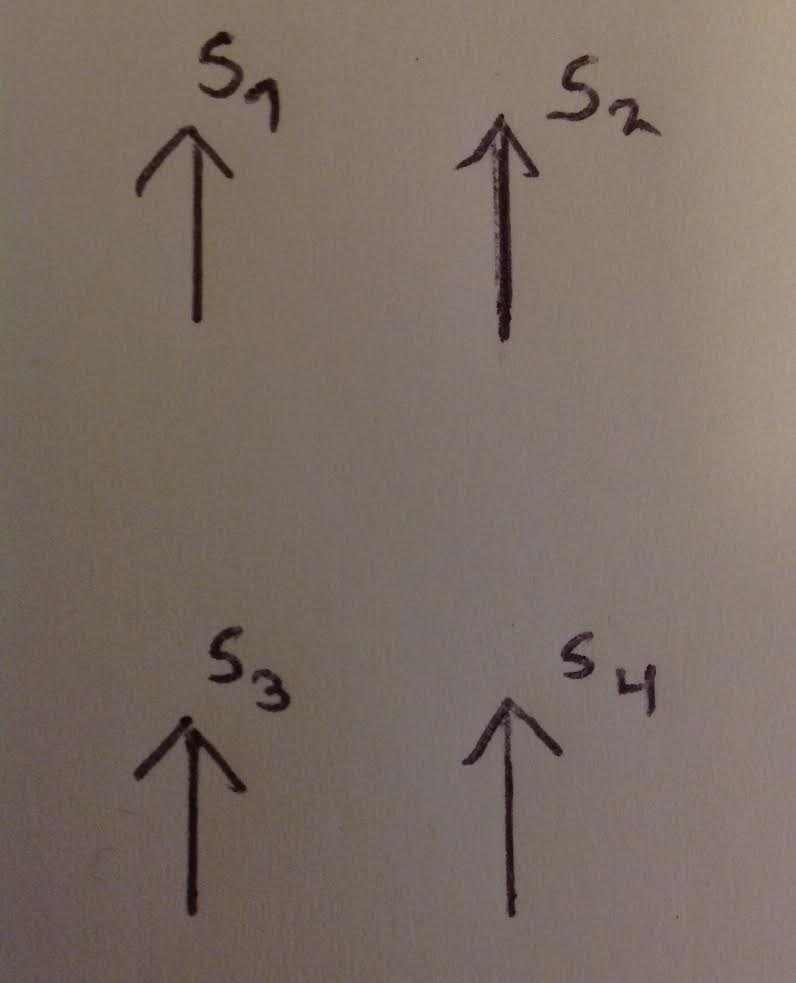
\includegraphics[scale=0.2]{SpinSystem.jpeg}
\caption{Labelling of our $2 \times 2$ lattice.}\label{fig:2x2spins}
\end{figure}
We begin with investigating the magnetization for the system. This is rather straightforward - we simply sum over all spins.\\
\linebreak
We now investigate the energy of each of the 16 microstates. We write the the energy as:
$$E=-J\left[s_1s_2+s_2s_1+s_1s_3+s_3s_1+s_2s_4+s_4s_2+s_3s_4+s_4s_3\right]$$
Let us now look at what happens for different spin arrangement. Let us first assume that all spins point upwards (+1). Then, the energy will be $E=-8J$. Similarly, if all spins point downwards (-1), the energy will be $E=8J$. If one spin points up, whilst all other point down, the energy will be zero, because half the terms change sign. Finally, if two spins point up, the energy depends on whether or not these spins neighbor each other. If they are next to each other, all terms involving the interaction of these two spins will have a positive sign. This will be two terms (notice that, because of the periodic boundary conditions, all interactions are reciprocal). The interaction between the two remaining spins will also be positive (as they have the same sign). However, all cross terms will give a negative contribution to the energy. Because of symmetry, these cross-terms must be the same as the not cross terms. Therefore the energy must be zero in this case. If, on the other hand, the two flipped spins are not neighbors, then there will be no interaction whatsoever between the flipped spins. Thus, all interacting spins have opposite signs, which gives the energy as $E=8J$. This is summarized in the following table:
\begin{center}
\begin{tabular}{|c|ccc|}
\hline
Spins up &Number of microstates&  Energy [J]& Magnetization[J/T]\\
\hline
4 & 1 &-8J&4\\
3 & 4 &0 & 2\\
2 &4 &0 &0 \\
2 & 2& 8J & 0\\
1 &4&+&6-2\\
0 & 1&-8J & -4 \\
\hline
\end{tabular}
\end{center}
Then we can define the microcanonical partition function as::
$$Z=\sum_{i=1}^{16} e^{-\beta E_i}$$
Calculations give:
$$Z=2e^{8\beta J}+2e^{-8\beta J} + 12$$
Or, recalling some hyperbolic trigonometric functions:
$$Z=4\cosh (8J\beta) +12$$
The energy is now given by:
\begin{equation}
\langle E \rangle = \sum_i \Delta E_i e^{-\beta \Delta E_i}
\end{equation}
Which gives, after some substantial but elementary algebra:
$$\frac{-16Je^{8\beta J}+16Je^{-8\beta J}}{2e^{8\beta J}+2e^{-8\beta J}+12}$$
Now $C_V$ is easy:
$$C_V=\frac{\langle E^2 \rangle - \langle E \rangle^2}{kT^2}$$
Where $\langle E^2 \rangle$ is:
$$\langle E^2\rangle=\frac{1}{Z} \sum_{i=1}^ {16}E_i^2e^{-\beta E_i}$$
The sum is easy:
$$\sum_{i=1}^{16}E_i^2e^{-\beta E_i}=128J^2\left(e^{8J\beta}+e^{-8J\beta}\right)$$
So that:
$$\langle E^2\rangle =\frac{256J^2\cosh(8J\beta)}{4\cosh(8J\beta)+12}$$
And thus:
\begin{equation}\label{eq:2x2Cv}
C_V=\frac{1}{kT}\left(\frac{256J^2\cosh(8J\beta)}{4\cosh(8J\beta)+12}-\left(\frac{-8J\sinh(8J\beta)}{\cosh(8J\beta)+3}\right)^2\right)
\end{equation}
Magnetization is easier, as it can be computed as:
$$\langle M \rangle=\frac{1}{Z}\sum_{i=1}^{16}M_ie^{-\beta E_i}$$
Which, however, gives:
$$\sum_{i=1}^{16}M_ie^{-\beta E_i}=4e^{8J\beta}+8-8-4e^{8J\beta}=0$$
$\langle \mathcal{M}^2\rangle$ can similarly be computed as:
$$\langle M^2 \rangle =\frac{8e^{8\beta J}+8}{\cosh(8J\beta)+3}$$
Now it is easy to compute the susceptibility:
\begin{equation}\label{eq:2x2Sus}
\chi = \frac{\langle M^2\rangle - \langle M \rangle^2}{kT}=\frac{1}{kT}\left(\frac{8e^{8\beta J}+8}{\cosh(8\beta J)+3}\right)
\end{equation}
Note, however, that we in application frequenty substitute $\langle \mathcal{M} \rangle$ with $\langle |\mathcal{M}|$ in place of $\angle \mathcal{M} \rangle$, for reasons explained \textbf{HERE}. Therefore, we also compute the expected value of the absolute value of the magnetization, which gives:
\begin{equation}\label{eq:2x2abs_mag}
\langle |M|\rangle =\frac{1}{Z}\sum_{i=1}^{16}|M_i|e^{-\beta E_i}=\frac{1}{Z}\left( 4e^{8J\beta}+4\cdot 2+ 4\cdot 2 +4e^{8J\beta}\right)=\frac{2e^{8J\beta}+4}{\cosh(8J\beta)+3}
\end{equation}

\subsection{A brief introducton to the Metropolis Algorithm}\label{Monte-Carlo_algo}
The Metropolis algorithm is very common in Monte Carlo simulations. It is an extremely elegant algorithm, based on the ratio of probabilities, as explained \textbf{HERE}. The idea is that the Boltzmann factor, $e^{-\beta \Delta E}$, tells us something about how probably it is to change state. If the energy difference bewteen the states is negative, the transition should be likely to occur, whereas if the energy difference is positive, it should be unlikely to occur. This is exactly what the Boltzmann factor expresses. The question is what to compare this factor to. This is at the heart of the simplest form of the Metropolis algorithm - simply choose a number, $a$ from a uniform distribtuion of values betweenn 0 and 1. Compare this number to $s^{-\beta J}$. If $a$ is less than $e^{-\beta J}$ (where  $\Delta E$ is the energy different between two states. If a is less than $e^{-\beta \Delta E}$, flip the spin. This simple recipe, surprisingly, gives the correct thermodynamic behavior as discussed \textbf{HERE.}

\subsection{Periodic boundary condition}
One problem of this model is how to treat the boundaries. The easiest way is to say that the spins on the boundaries have no neighbors. Real materials have close to infinite atom spins, so the boundaries are negligible. But we can't simulate infinite lattices, so we have to find another. With periodic boundary conditions, the spins at the boundary treats the spins at the opposite boundary as its neighbor. This will make a good approximation to an infinite lattice, since every spin has a neighbor. Because of this does the boundary condition corresponds better with reality.








\section{Methods}
\subsection{Finding the Energy}\label{energy_in_system}
The fastest and easiest way of implement the Ising method is to flip one spin at the time. This is because the energy difference $\Delta E$ in the system only will depend on the energy difference on a single spin. $\Delta E$ of a spin only depends on its closest neighbors, and can only have one of five values:

$$\Delta E = \{ -8J, -4J, 0, 4J, 8J\}$$

This means that all the values for $e^{\beta \Delta E}$ can be precomputed. This saves us a lot of this in large simulations.\\

For each spin flip, we calculate the $\Delta E$ by checking the spin of the neighbor spins, and using \ref{metropolis_algo_implementation}.

Before starting the Metropolis algorithm the energy of the system has to be calculated this is done by looping though all the spins and calculating:

\lstinputlisting{Pseudo_code_total_energy.cpp}

\subsection{The Periodic Boundary Conditions}
The easiest way of implementing the boundary conditions is with modular division. Every time we want to calculate $\Delta E$, we have to use four nearest neighbors, but this neighbor may not exist. If the spin we are calculating $\Delta E$ is $x_{N-1}$, then its neighbor $x_{N}$ does not exit. Instead we will check $periodic({N})$, where 

\begin{equation}
periodic(i) = (i + N) \text{mod} N
\end{equation} 

We can check this we can test with $periodic(N)$ which should be $0$

\begin{equation}
periodic(N) = (N + N)\text{mod} N = 0
\end{equation}

So as we can see this loops to the other side of the lattice. 



\subsection{Implementing the Metropolis algorithm}\label{metropolis_algo_implementation}
We implemented the Metropolis algorithm by looping over two nested for-loops. The outer for-loop loops over the number of Monte Carlo cycles, while the inner loops over the number if spin. Inside the loops a spin in the lattice is chosen to be flipped. The then energy difference is calculated from 

$$\Delta E = 2J\sum_k s_is_k$$

we use this to to find the precalculated Boltzmann factor, and compare this with a random variable $\zeta \in [0,1]$, as described in \ref{Monte-Carlo_algo}, and check if this flip is acceptable.\\

Here is psudo-code describing the implementation of the Metropolis algorithm. Periodic boundary conditions are not implemented:
 
\lstinputlisting{Pseudo_code_Metropolis.cpp}

\subsection{Investigating the time to reach at the most likely state, and probability distribution}

We are interested in seeing how long it takes the system to reach the most likely state, and if this depends on the temperature. We also wish to see if the start configuration change this time. We want to check when the mean energy and the mean absolute value of the magnetization smooth out and converges to a value. Since is difficult to do in a qualitative way, so we are just going to plot these values against the Monte Carlo cycles, and look for the cycle where this happens. We will also look at the number of accepted flips, since, as discussed in section \ref{equilibrium_system}, we also want the accepted flips to converge as we reach equilibrium.\\

We also want to look at the probability distribution of the equilibrium state. This is done by counting the number of times a certain $E$ appears. We then have to use what we found above, and start when the equilibrium state is started.

\subsection{The Phase transitions}
We already have an analytical temperature for $T_C(N=\infty)$ from section \ref{phase_tranisition}, $\sim 2.269 K$. We are there for only going to look at temperatures in an interval around this temperature while investigating the phase transitions. At the critical temperature the heat capacity and the magnetic susceptibility are going to diverge, but since we are using finite lattices, they aren't going to go to diverge, but they are going to show a value much higher then for the surrounding. This spike will give the critical temperature, which we can compare with the equations from section \ref{phase_tranisition}.


\subsection{Parallelizing with MPI}
Monte Carlo methods have an error(variance) 

$$
\sigma \sim \frac{1}{\sqrt{N}}
$$

This means that the higher the number of cycles we use, the more accurate the simulation will be. One way of getting more cycles without increasing the run time is with parallelization. MPI lets us use all the core of the CPU. The Monte Carlo calculation as sent to the cores, and when the they are done they(the slaves) will send to data to a master core/node. This node will find calculate the mean of all the data. We are mainly using 4 cores, so with MPI, we will get 4 times the Monte Carlo cycles, and more accurate data. \footnote{Note that we initially intended to run on a larger cluster but, due to time constraints, this was not possible.}

\section{Results}

\subsection{Numerical vs Analytical results for a 2 $\times$ 2 lattice}

Before going on to larger lattices, we want to check if out program works. The one system we have an analytical results for are the 2x2 \ref{2x2analytic}. We want to look at how many Monte Carlo cycles it take to get a numerical result which corresponds well to the analytical. The most characteristic quantity is the heat capacity, so we choose to use this for the comparison. To make the plots as general as possible, all quantities  are per spin.

\begin{figure}[!ht]
    \centering
    \begin{subfigure}[H!]{0.5\textwidth}
        \centering
        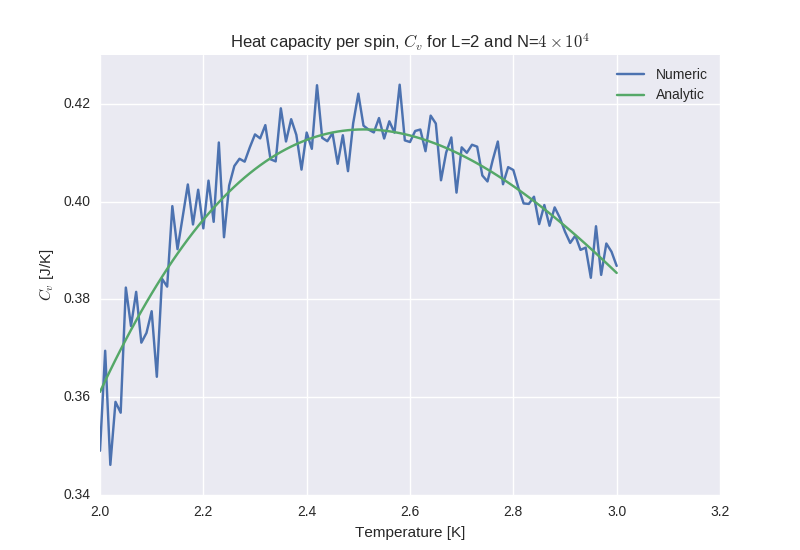
\includegraphics[height=2.2in]{L2Cv4e4.png}
        \caption{$N=4\times 10^4$}
    \end{subfigure}%
    ~ 
    \begin{subfigure}[H!]{0.5\textwidth}
        \centering
        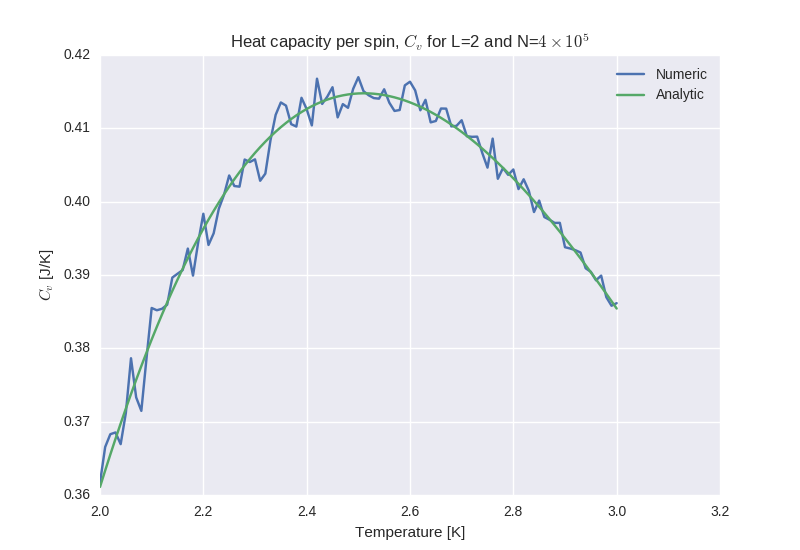
\includegraphics[height=2.2in]{L2Cv4e5.png}
        \caption{$N=4\times 10^5$}
    \end{subfigure}
    \begin{subfigure}[H!]{0.5\textwidth}
        \centering
        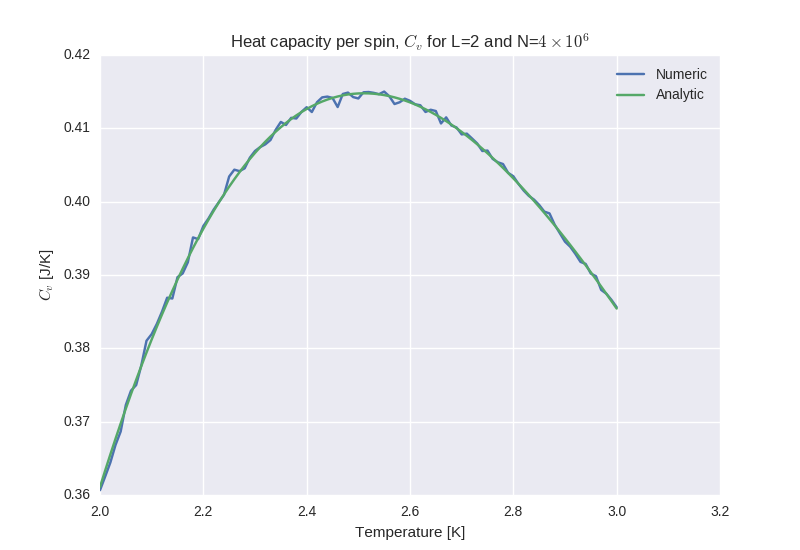
\includegraphics[height=2.2in]{L2Cv4e6.png}
        \caption{$N=4\times 10^6$}
    \end{subfigure}%
    ~ 
    \begin{subfigure}[H!]{0.5\textwidth}
        \centering
        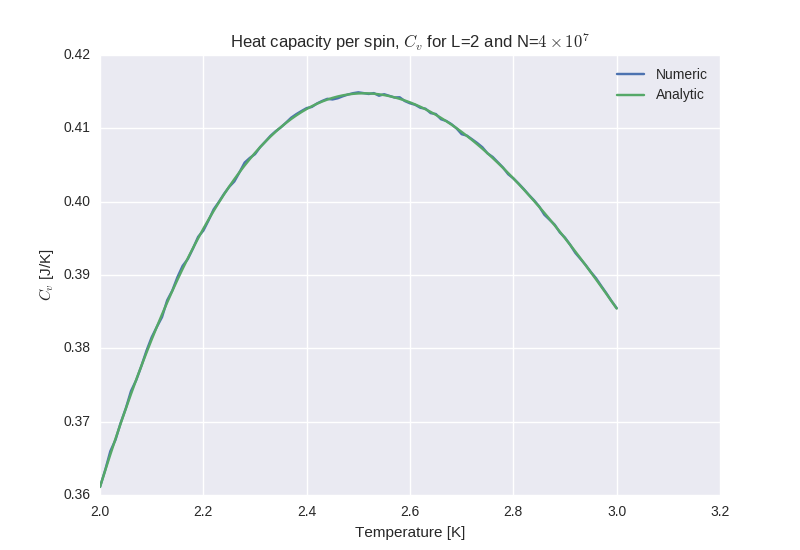
\includegraphics[height=2.2in]{L2Cv4e7.png}
        \caption{$N=4\times 10^7$}
    \end{subfigure}
    \caption{Comparison of the numeric and analytic solution of heat capacity and mean energy per spin for the $2\times 2$ lattice. We plot multiple Monte Carlo steps, $N$, to find where the correspondence becomes good. This was done with temperatures in the interval $kT/J=2$ to $kT/J=3$, with 10 steps inbetween.}\label{fig:2x2_nsteps}
\end{figure}


We gave each core a $N = 10^n$, with 4 cores, this means that our simulation runs with  $N = 4 \times 10^n$ cycles. We see from the plots that if use $N = 4 \times 10^7$, we get a very good correspondence between the analytic and the numeric solution. We will therefor plot the other thermodynamic quantities in the $2\times 2$ lattice for this value of $N$. 

\begin{figure}[!ht]
    \centering
    \begin{subfigure}[H!]{0.5\textwidth}
        \centering
        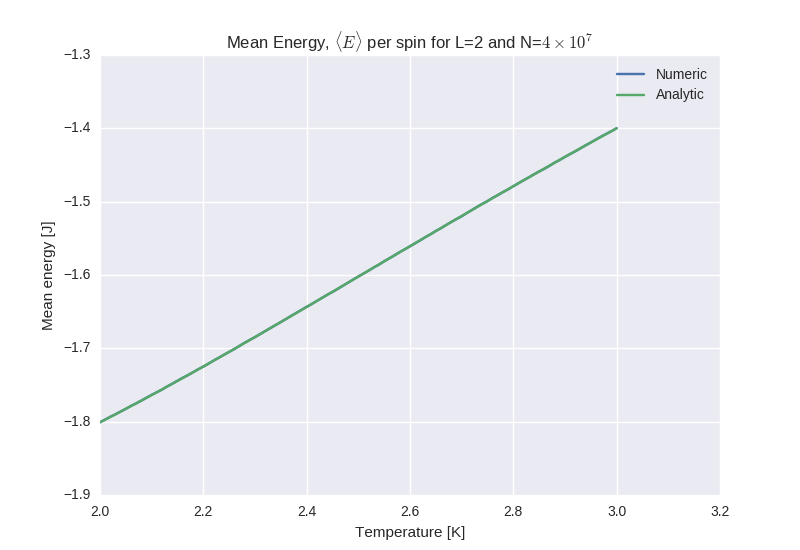
\includegraphics[height=2.2in]{L2MeanEner4e7.png}
        \caption{Mean energy per spin}
    \end{subfigure}%
    ~ 
    \begin{subfigure}[H!]{0.5\textwidth}
        \centering
        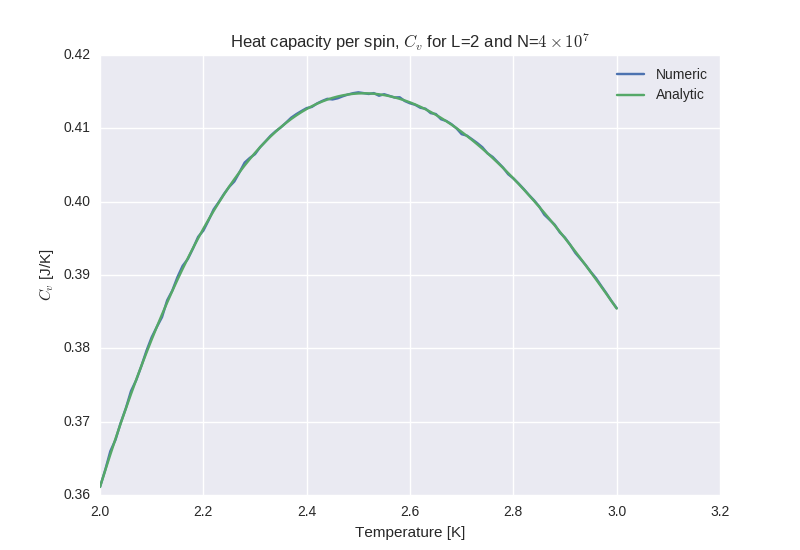
\includegraphics[height=2.2in]{L2Cv4e7.png}
        \caption{Heat capacity per spin}
    \end{subfigure}
    ~
     \begin{subfigure}[H!]{0.5\textwidth}
        \centering
        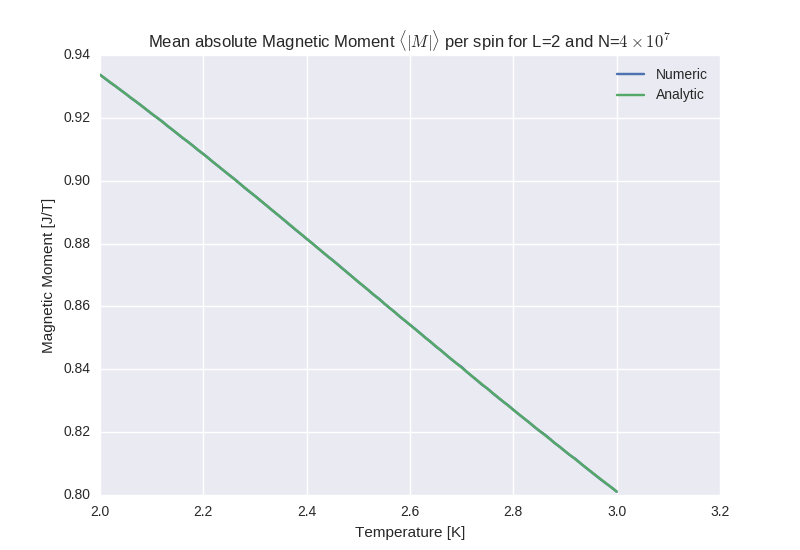
\includegraphics[height=2.2in]{L2MeanabsMag4e7.png}
        \caption{Mean absolute magnetic moment per spin}
    \end{subfigure}%
    ~ 
    \begin{subfigure}[H!]{0.5\textwidth}
        \centering
        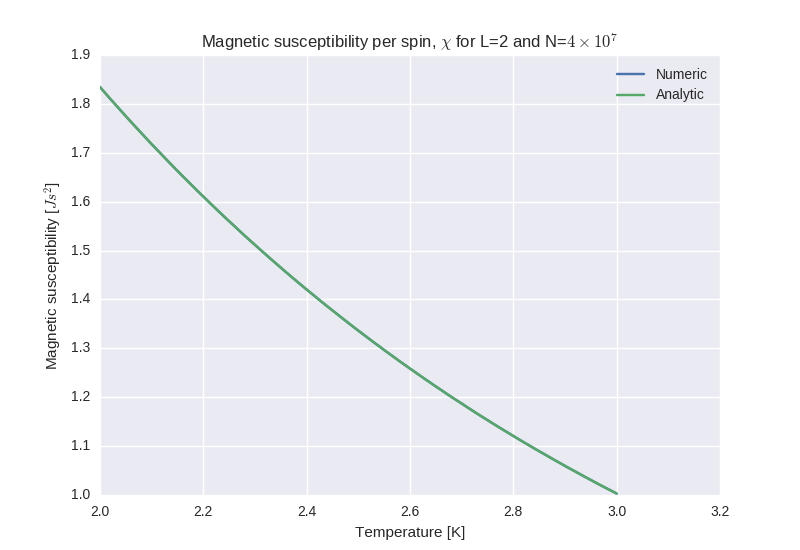
\includegraphics[height=2.2in]{L2MagSus4e7.png}
        \caption{Magnetic susceptibility per spin}
    \end{subfigure}
    \caption{Comparison of the numeric and  analytic solution for the mean energy per spin, heat capacity per spin, mean absolute magnetic moment per spin and magnetic susceptibility of the $2 \times 2$ lattice, running $10^7$ Monte Carlo cycles for each temperature. }\label{fig:2x2_thermo}
\end{figure}
\subsection{Results from our investigation into the equilibration time}
We were now interested in find the $N$ were the equilibrium state is reach. For this we used a larger lattice, $20 \times 20$ spins. We are going to start with a temperature of $kT/J=1.0$. We are interested in seeing where the quantities converges to there equilibrium value. We want to look at both the random and homogenous start. Here are the plots of mean energy and mean absolute value of the magnetization: 

\begin{figure}[!ht]
    \centering
    \begin{subfigure}[H!]{0.5\textwidth}
        \centering
        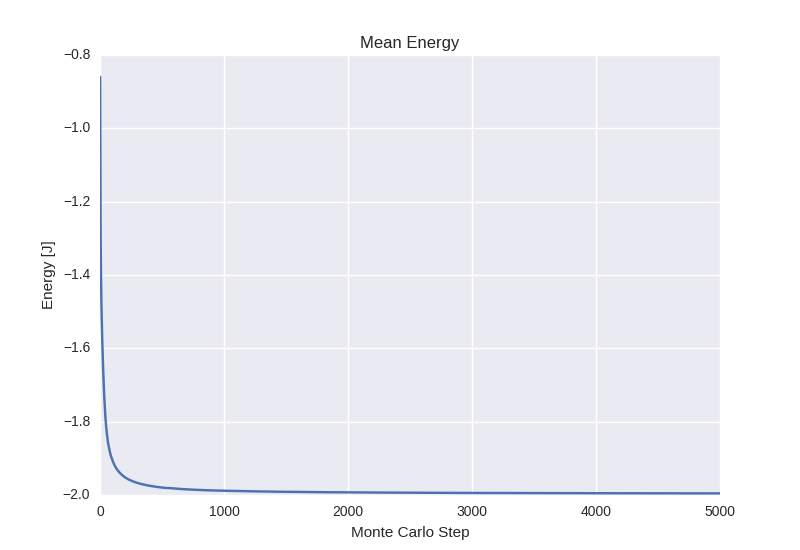
\includegraphics[height=2.2in]{meanEnergyWRandomStart.png}
        \caption{Mean energy per spin from disordered state}
    \end{subfigure}%
    ~ 
    \begin{subfigure}[H!]{0.5\textwidth}
        \centering
        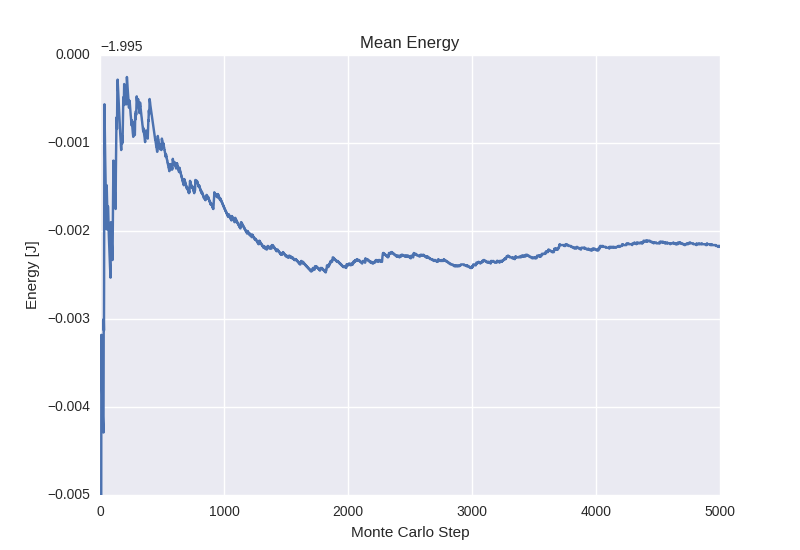
\includegraphics[height=2.2in]{meanEnergyWUpStart.png}
        \caption{Mean energy per spin from uniform state}
    \end{subfigure}
        ~
     \begin{subfigure}[H!]{0.5\textwidth}
        \centering
        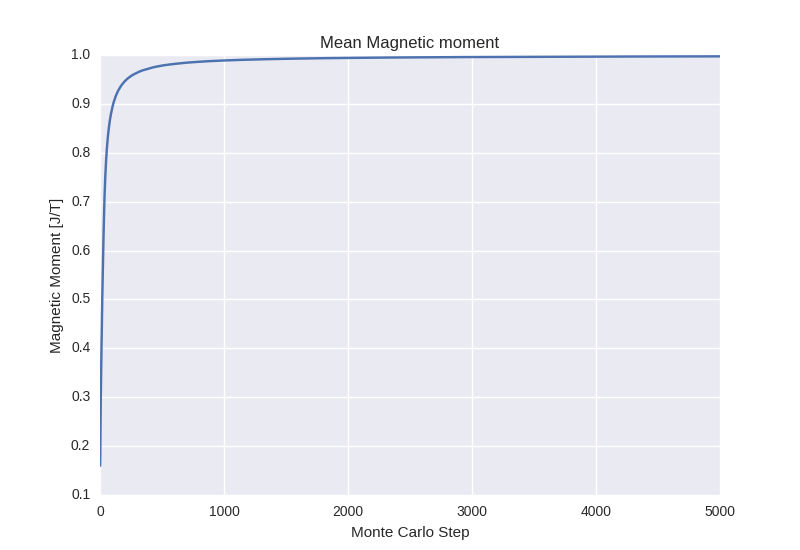
\includegraphics[height=2.2in]{meanMagMomWRandomStart.png}
        \caption{Mean absolute magnetic moment per spin from disordered state}
    \end{subfigure}%
    ~ 
    \begin{subfigure}[H!]{0.5\textwidth}
        \centering
        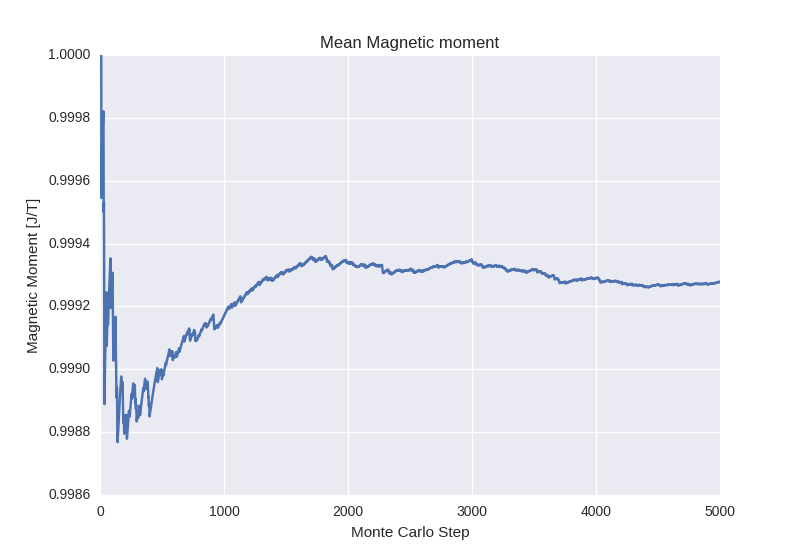
\includegraphics[height=2.2in]{meanMagMomWUpStart.png}
        \caption{Mean absolute magnetic moment per spin from uniform state}
    \end{subfigure}
      \caption{Time development of mean energy and mean magic moment per spin for two different initial configurations.Here $L=20$ and $kT/J=1.0$.}\label{fig:20x20_Sweep_T_1}
\end{figure}
We also plot the same quantities for a temperature of $kT/J=2.4$ in the figure below:
\begin{figure}[!ht]
    \centering
    \begin{subfigure}[H!]{0.5\textwidth}
        \centering
        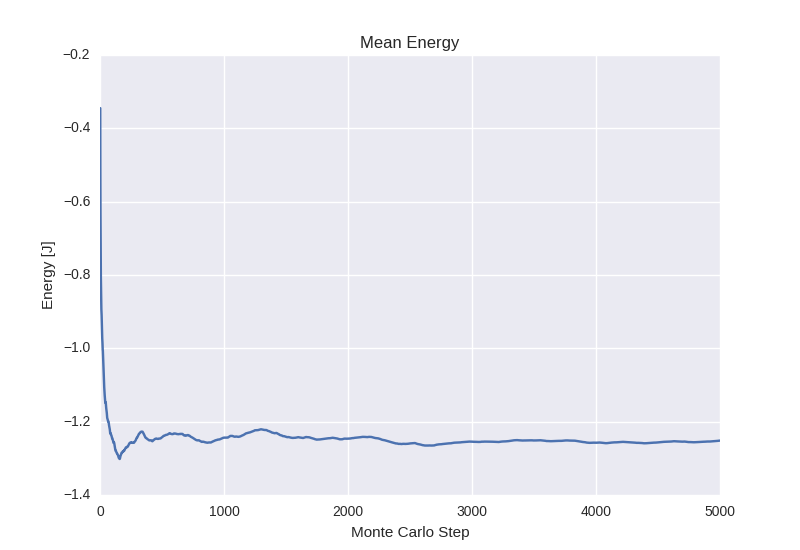
\includegraphics[height=2.2in]{meanEnergyWRandomStartT24.png}
        \caption{Mean energy per spin from disordered state}
    \end{subfigure}%
    ~ 
    \begin{subfigure}[H!]{0.5\textwidth}
        \centering
        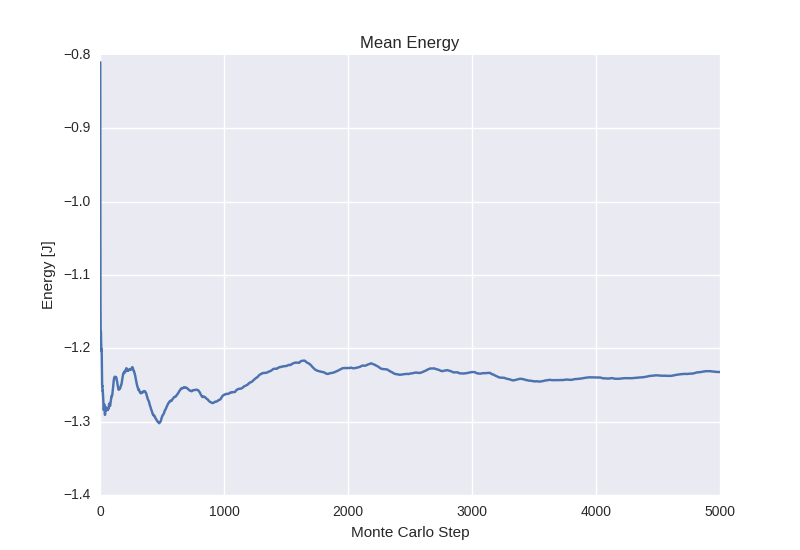
\includegraphics[height=2.2in]{meanEnergyWUpStartT24.png}
        \caption{Mean energy per spin from uniform state}
    \end{subfigure}
        ~
     \begin{subfigure}[H!]{0.5\textwidth}
        \centering
        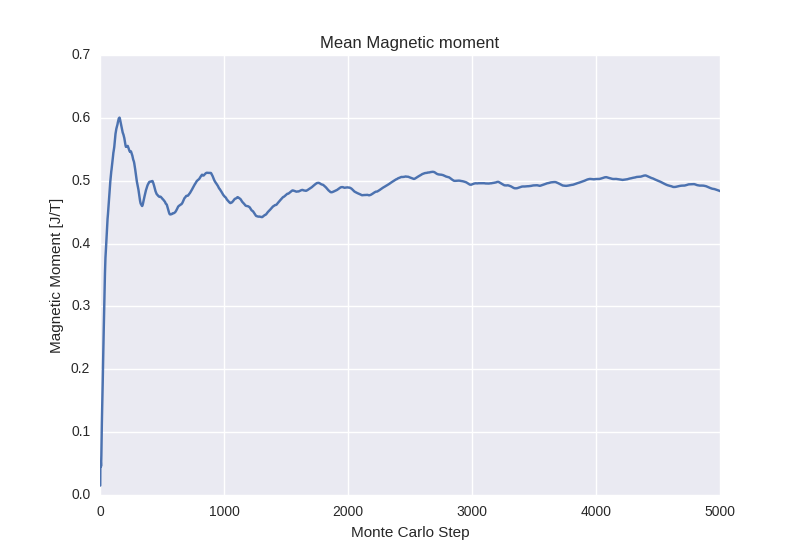
\includegraphics[height=2.2in]{meanMagMomWRandomStartT24.png}
        \caption{Mean absolute magnetic moment per spin from disordered state}
    \end{subfigure}%
    ~ 
    \begin{subfigure}[H!]{0.5\textwidth}
        \centering
        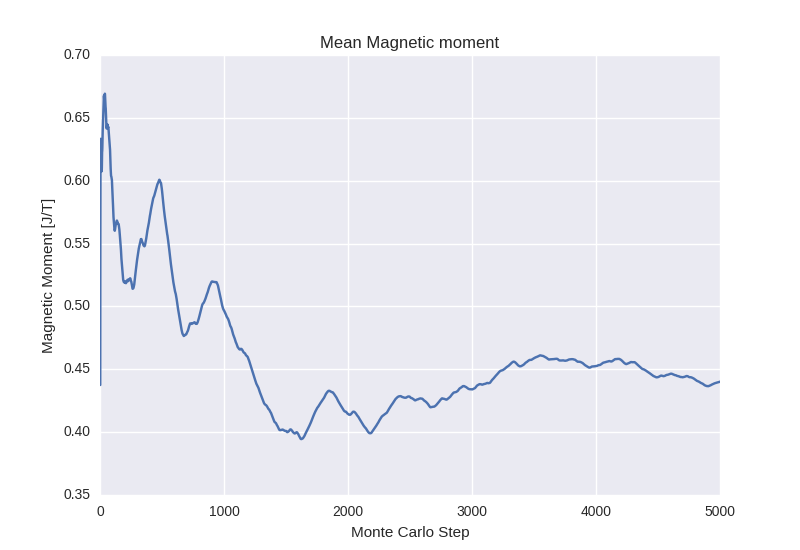
\includegraphics[height=2.2in]{meanMagMomWUpStartT24.png}
        \caption{Mean absolute magnetic moment per spin from uniform start}
    \end{subfigure}
      \caption{Time development of mean energy and mean magic moment per spin for two different initial configurations. Here $L=20$ and $kT/J=2.4$.}\label{fig:20x20_Sweep_T_24}
\end{figure}

Finally, we also plot the number of accepted flips per spin and time, to get a sense of how many spins the Metropolis algorithm flips at every time step. We do this for two different temperatures, again using both an ordered and a disordered state.
\begin{figure}[!ht]
    \centering
    \begin{subfigure}[H!]{0.5\textwidth}
        \centering
        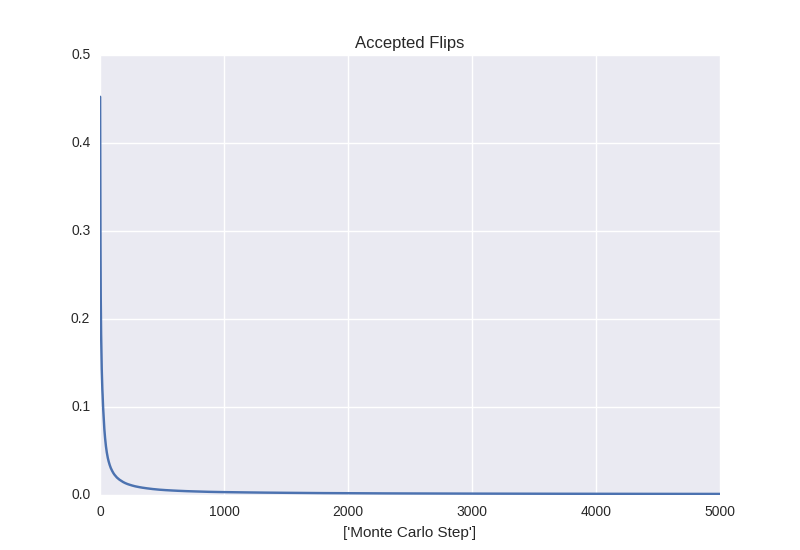
\includegraphics[height=2.2in]{flipsWRandomStart.png}
        \caption{With disordered initial state, at $kT/J=1$}
    \end{subfigure}%
    ~ 
    \begin{subfigure}[H!]{0.5\textwidth}
        \centering
        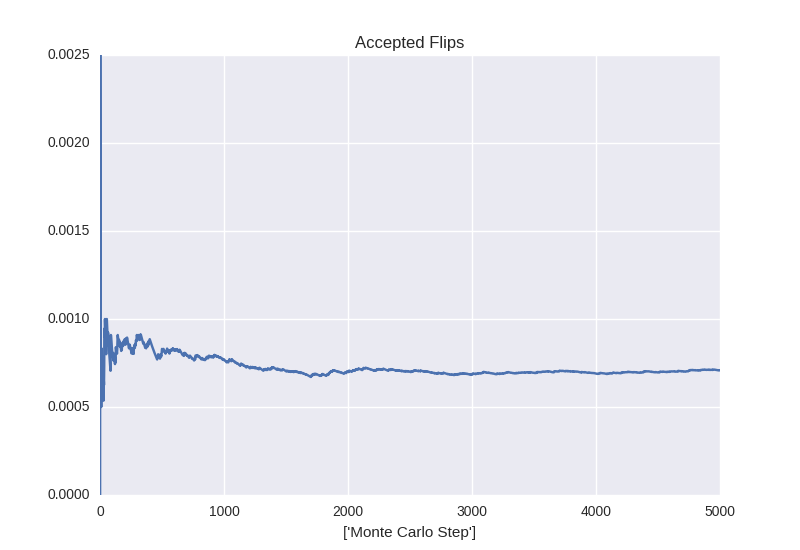
\includegraphics[height=2.2in]{flipsWUpStart.png}
        \caption{With uniform initial state, at $kT/J=1$}
    \end{subfigure}
        ~
     \begin{subfigure}[H!]{0.5\textwidth}
        \centering
        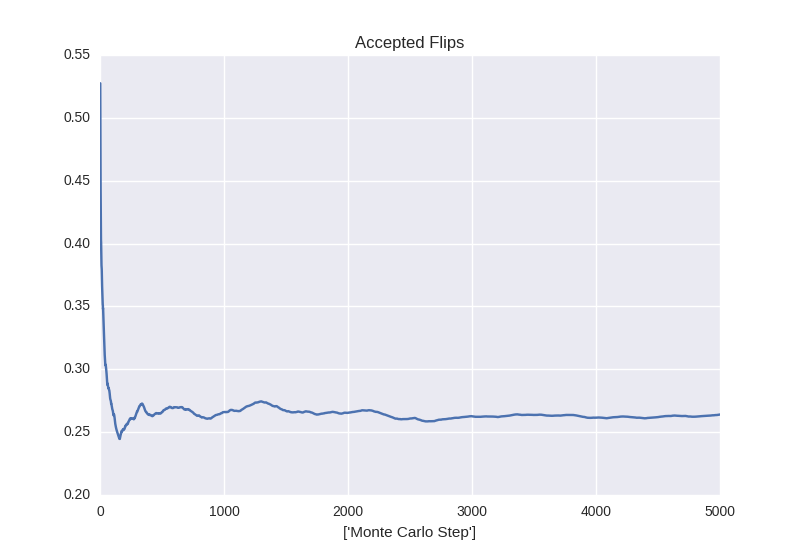
\includegraphics[height=2.2in]{flipsWRandomStartT24.png}
        \caption{With disordered initial state, at $kT/J=2.4$}
    \end{subfigure}%
    ~ 
    \begin{subfigure}[H!]{0.5\textwidth}
        \centering
        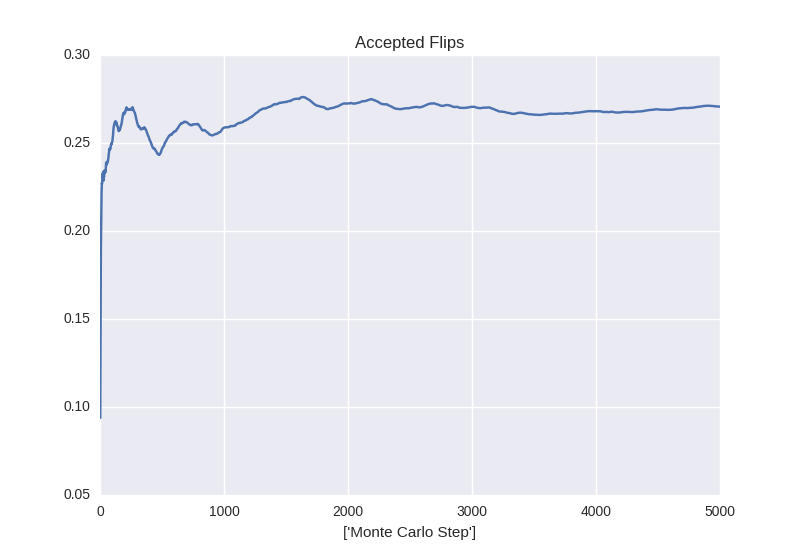
\includegraphics[height=2.2in]{flipsWUpStartT24.png}
        \caption{With uniform initial state, at $kT/J=2.4$}
    \end{subfigure}
      \caption{Mean number of accepted flips per spin per Monte Carlo cycle for different initial states and different temperatures.}\label{fig:20x20_Sweep_flips}
\end{figure}
All these figures seem to indicate that equilibrium is quickly reached (after less than 2000 cycles). However, sometimes this is not the case, as we hit a local minimum (described in more detail \textbf{HERE}). This gives the following plots:


\begin{figure}[!ht]
    \centering
    \begin{subfigure}[H!]{0.5\textwidth}
        \centering
        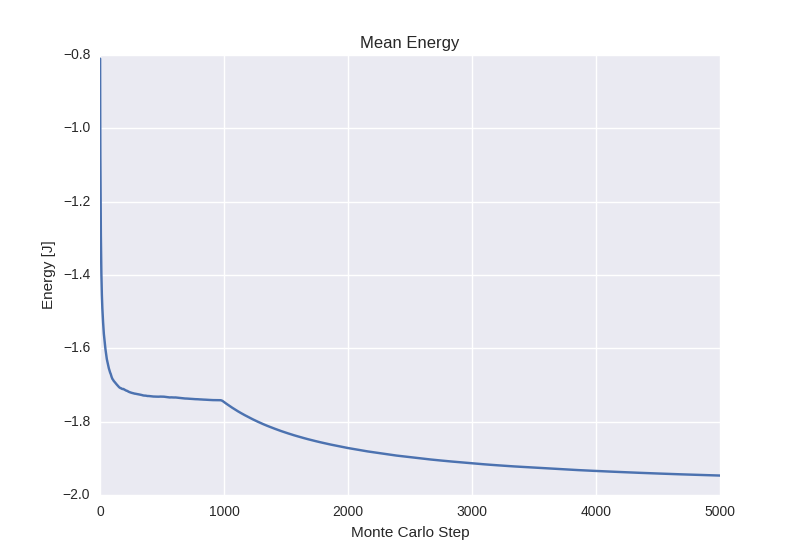
\includegraphics[height=2.2in]{meanEnergyLocalMin.png}
        \caption{Mean energy per spin from uniform state}
    \end{subfigure}%
    ~ 
    \begin{subfigure}[H!]{0.5\textwidth}
        \centering
        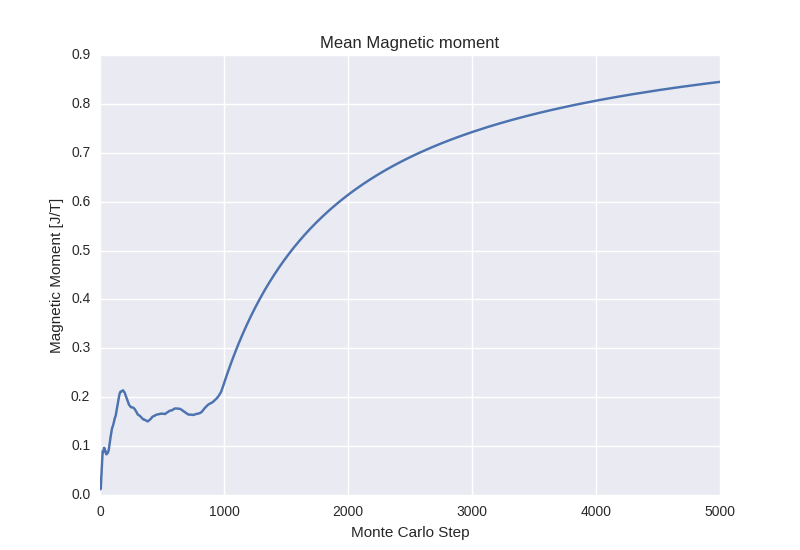
\includegraphics[height=2.2in]{meanMagMomLocalMin.png}
        \caption{Mean magnetic moment per spin from uniform state}
    \end{subfigure}
     ~ 
    \begin{subfigure}[H!]{0.5\textwidth}
        \centering
        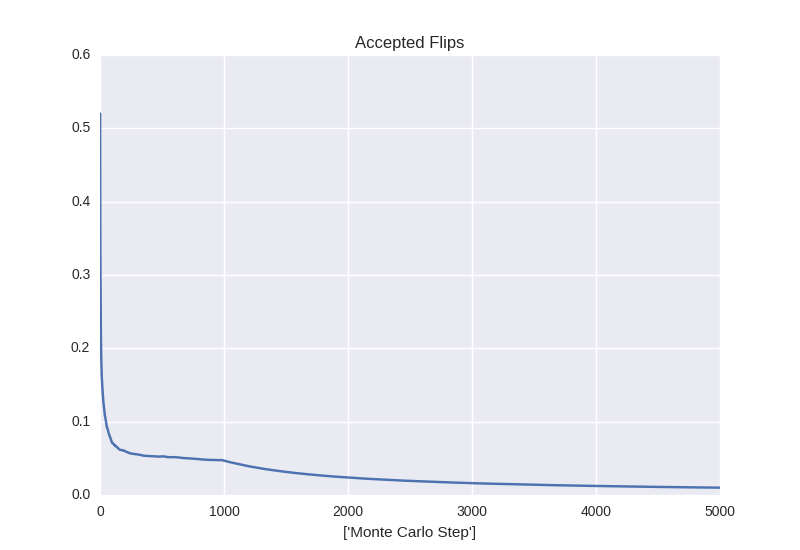
\includegraphics[height=2.2in]{flipsLocalMin.png}
        \caption{Mean number of accepted flips per spin per Monte Carlo cycle from uniform state}
    \end{subfigure}
       \caption{Time development of mean energy, mean magnetic moment and mean number of accepted flips per spin per Monte Carlo cycle for a system with $L=20$, $kT/J=1$, with all spins initially pointing up.}\label{fig:20x20_Sweep_flips}
\end{figure}
This shows that it sometimes takes significantly longer to arrive at equilibrium. Furthermore, equilibration time may also increase for higher temperature. Therefore, we choose 5000 Monte Carlo cycles as a safe equilibration time.
\subsection{Results from our investigation into the probability distribution}
Here we plot the probability of a certain energy occurring for two different temperatures. We plot this both as a curve and as a histogram.
\begin{figure}[!ht]
    \centering
    \begin{subfigure}[H!]{0.5\textwidth}
        \centering
        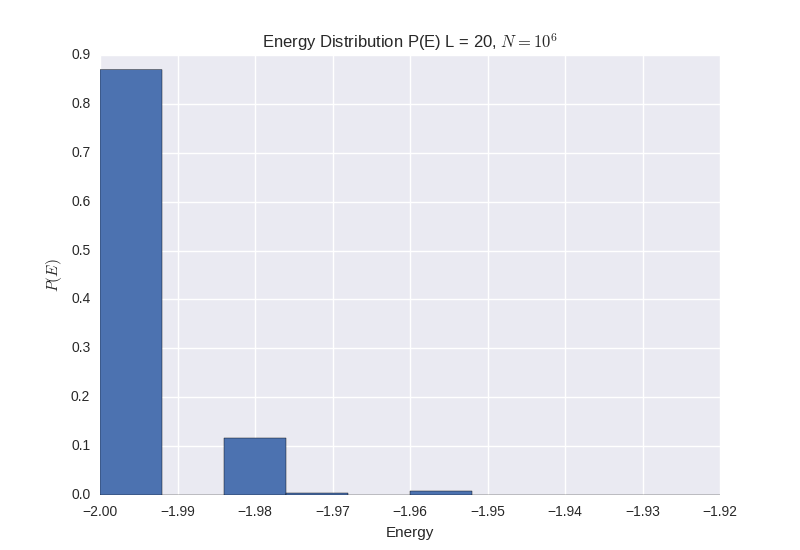
\includegraphics[height=2.2in]{energyDistHistoT1.png}
        \caption{$KT/J=1$}
    \end{subfigure}%
    ~ 
    \begin{subfigure}[H!]{0.5\textwidth}
        \centering
        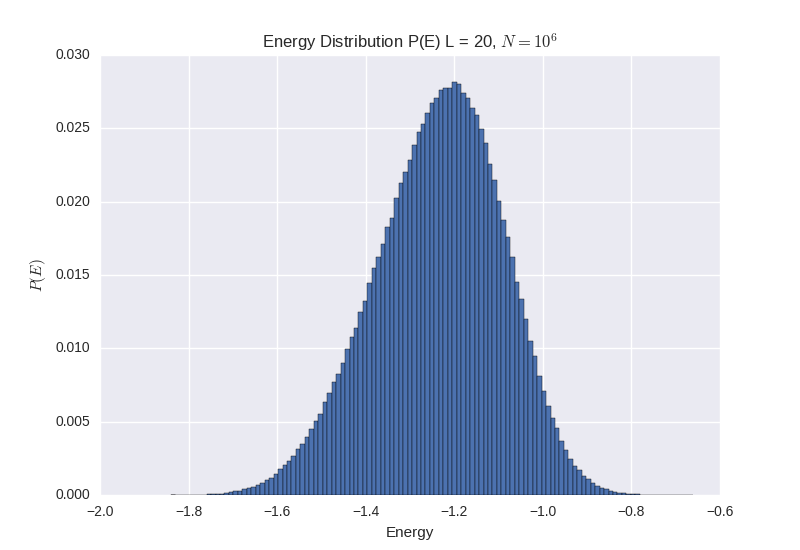
\includegraphics[height=2.2in]{energyDistHisto.png}
        \caption{$KT/J=2.4$}
    \end{subfigure}
       \caption{Histogram showing the probability of different energies occurring for two different temperature. This is for a lattice with $L=20$, simulated with $N=10^5$ Monte Carlo cycles, excluding an equilibration time of 5000 cycles. }
\end{figure}

\subsection{Results from our investigation of phase transitions}
Here, we wish to investigate how the critical temperature, which we extract by looking at the susceptibility and heat capacity, depends on our lattice size $L$. We also include the mean energy and the absolute value of the mean magnetization for completeness. 
\begin{figure}[!ht]
    \centering
    \begin{subfigure}[H!]{0.5\textwidth}
        \centering
        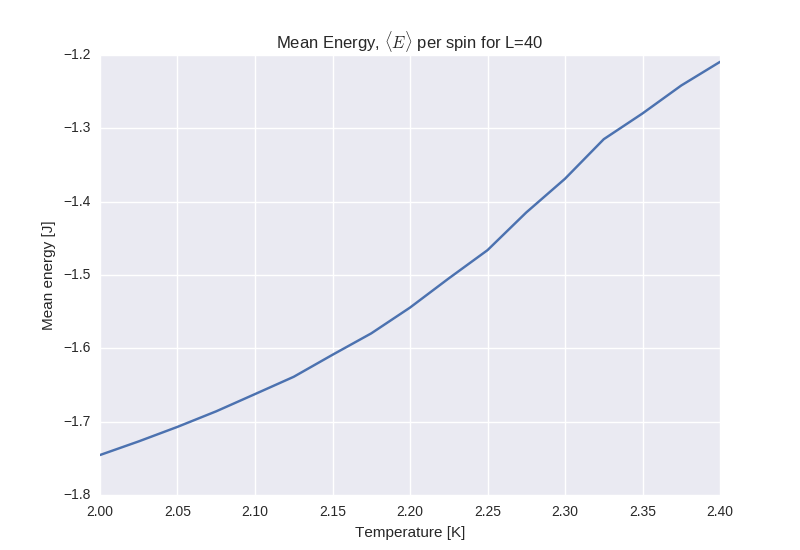
\includegraphics[height=2.2in]{meanEnergyl40Ne5New.png}
        \caption{Mean energy per spin for $L=40$}
    \end{subfigure}%
    ~ 
    \begin{subfigure}[H!]{0.5\textwidth}
        \centering
        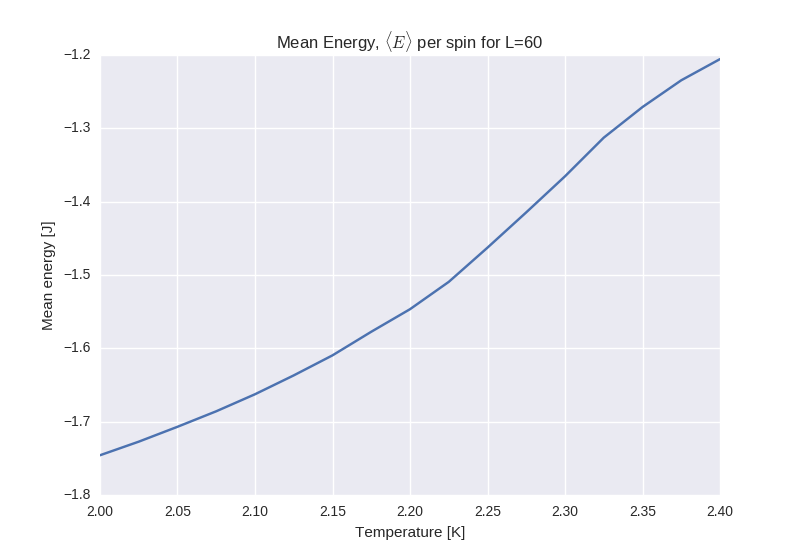
\includegraphics[height=2.2in]{meanEnergyl60Ne5New.png}
        \caption{Mean energy per spin for $L=60$}
    \end{subfigure}
        ~
     \begin{subfigure}[H!]{0.5\textwidth}
        \centering
        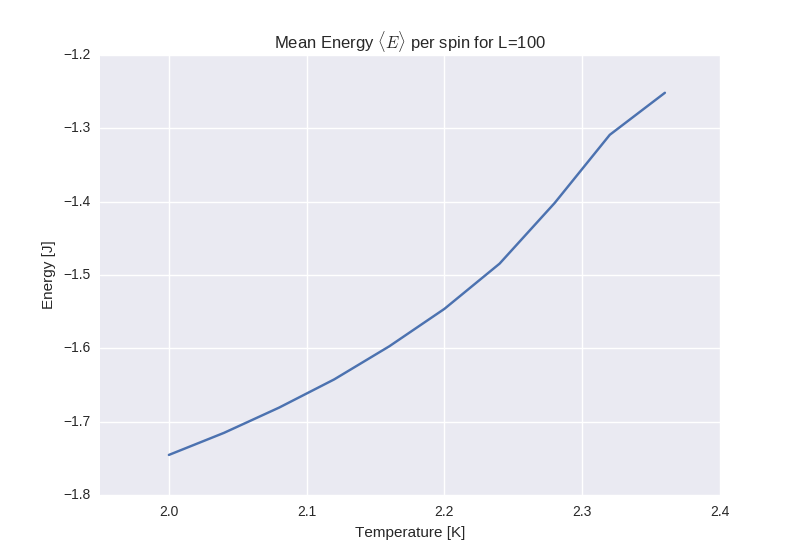
\includegraphics[height=2.2in]{meanEnergyl100Ne5New.png}
        \caption{Mean energy per spin for $L=100$}
    \end{subfigure}%
    ~ 
    \begin{subfigure}[H!]{0.5\textwidth}
        \centering
        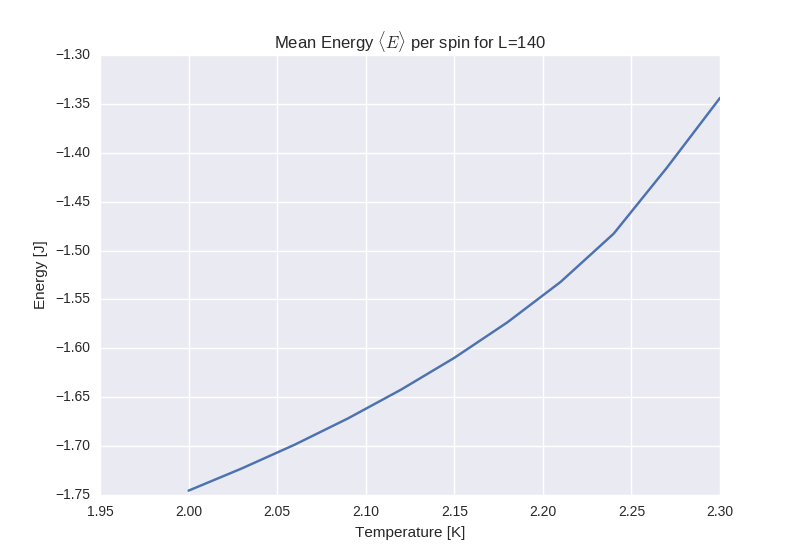
\includegraphics[height=2.2in]{meanEnergyl140.png}
        \caption{Mean energy per spin for $L=140$}
    \end{subfigure}
      \caption{Development of the mean energy per spin for systems of different sizes, as a function of temperature. We simulated $10^5$ Monte Carlo cycles, excluding an equilibration time of 5000 cycles.}
\end{figure}
\begin{figure}[!ht]
    \centering
    \begin{subfigure}[H!]{0.5\textwidth}
        \centering
        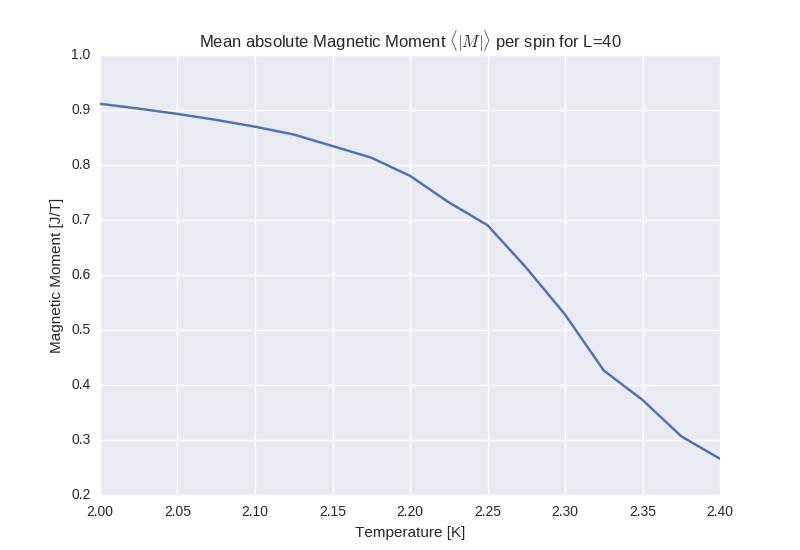
\includegraphics[height=2.2in]{meanMagMoml40Ne5New.png}
        \caption{Mean absolute value of the magnetic moment per spin for $L=40$}
    \end{subfigure}%
    ~ 
    \begin{subfigure}[H!]{0.5\textwidth}
        \centering
        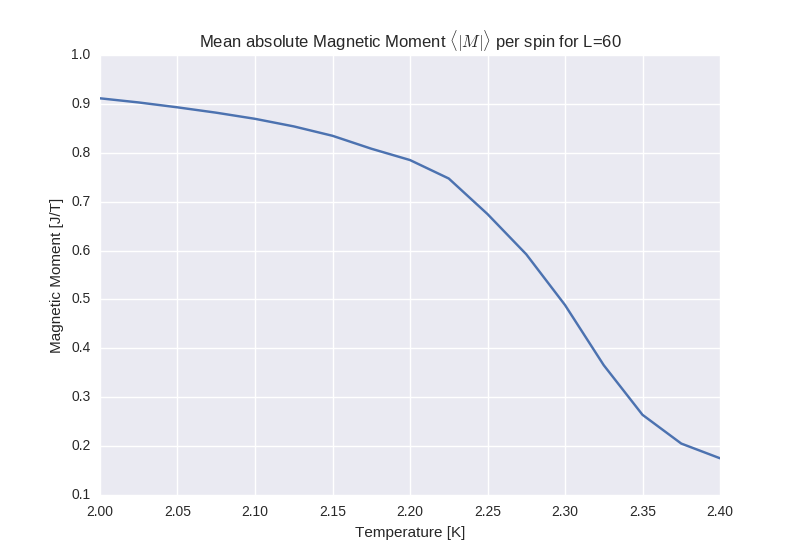
\includegraphics[height=2.2in]{meanMagMoml60Ne5New.png}
        \caption{Mean absolute value of the magnetic moment per spin for $L=60$}
    \end{subfigure}
        ~
     \begin{subfigure}[H!]{0.5\textwidth}
        \centering
        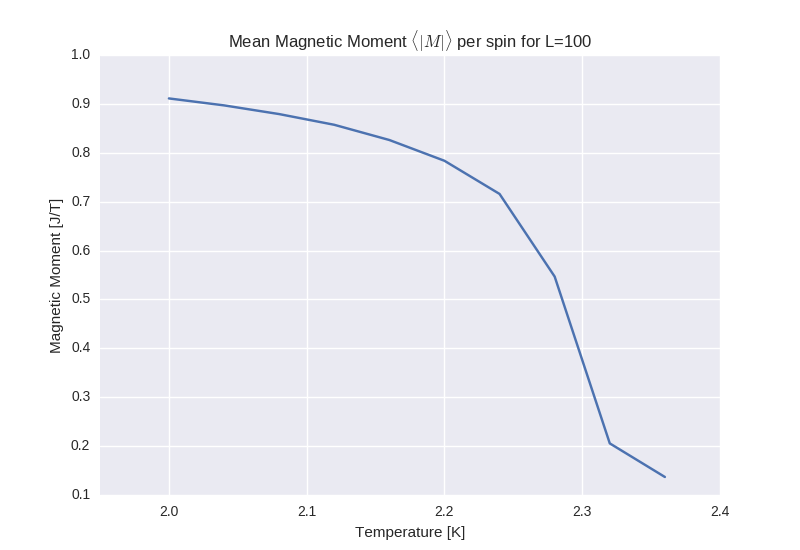
\includegraphics[height=2.2in]{meanMagMoml100Ne5New.png}
        \caption{Mean absolute value of the magnetic moment per spin for $L=100$}
    \end{subfigure}%
    ~ 
    \begin{subfigure}[H!]{0.5\textwidth}
        \centering
        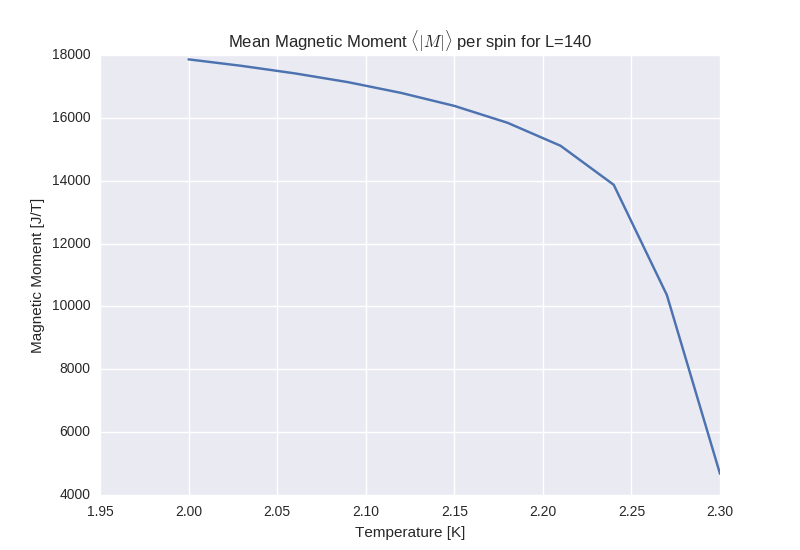
\includegraphics[height=2.2in]{meanMagMoml140.png}
        \caption{Mean absolute value of the magnetic moment per spin for $L=140$}
    \end{subfigure}
      \caption{Development of the mean absolute value of the magnetic moment per spin for systems of different sizes, as a function of temperature. We simulated $10^5$ Monte Carlo cycles, excluding an equilibration time of 5000 cycles.}
\end{figure}
\begin{figure}[!ht]
    \centering
    \begin{subfigure}[H!]{0.5\textwidth}
        \centering
        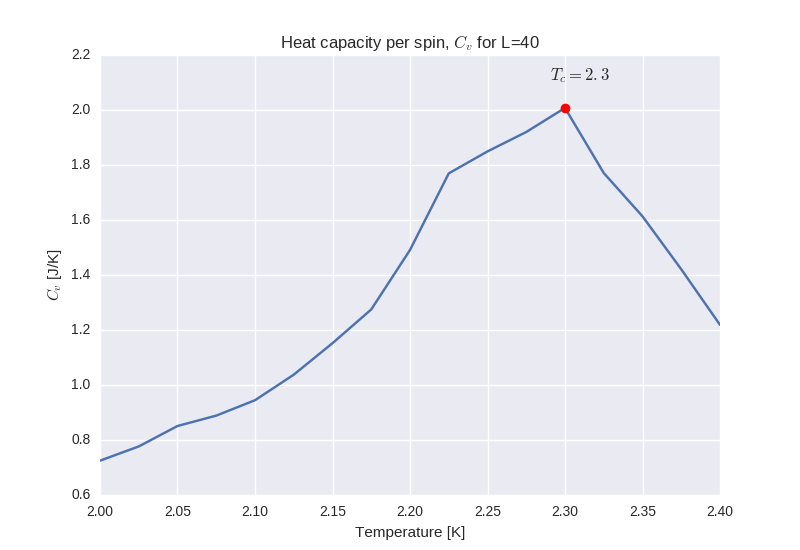
\includegraphics[height=2.2in]{cvl40Ne5New.png}
        \caption{Heat capacity for $L=40$}
    \end{subfigure}%
    ~ 
    \begin{subfigure}[H!]{0.5\textwidth}
        \centering
        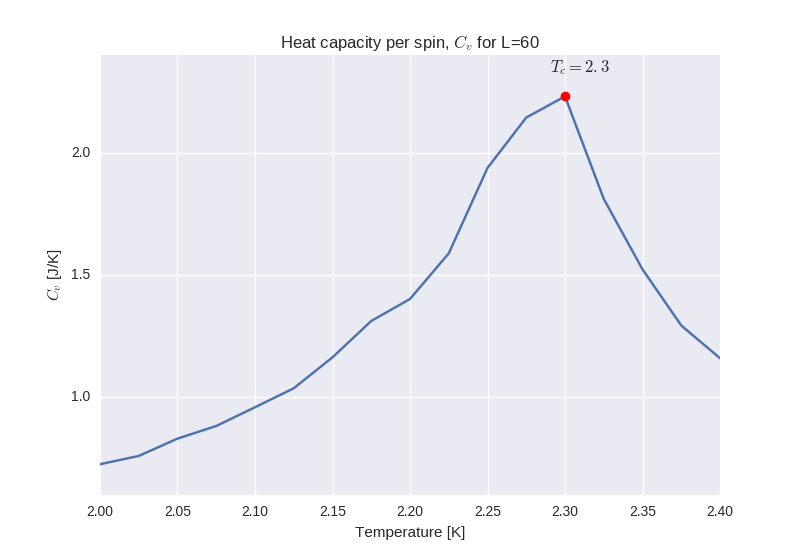
\includegraphics[height=2.2in]{cvl60Ne5New.png}
        \caption{Heat capacity for $L=60$}
    \end{subfigure}
        ~
     \begin{subfigure}[H!]{0.5\textwidth}
        \centering
        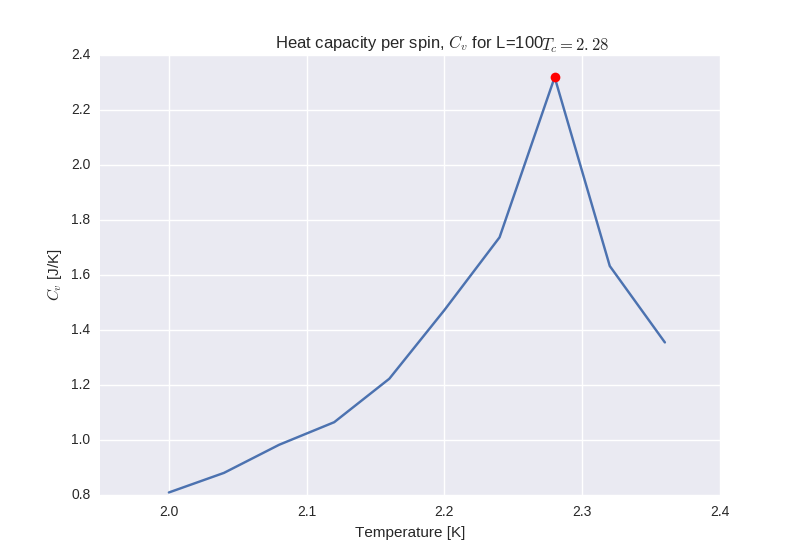
\includegraphics[height=2.2in]{cvl100Ne5New.png}
        \caption{Heat capacity for $L=100$}
    \end{subfigure}%
    ~ 
    \begin{subfigure}[H!]{0.5\textwidth}
        \centering
        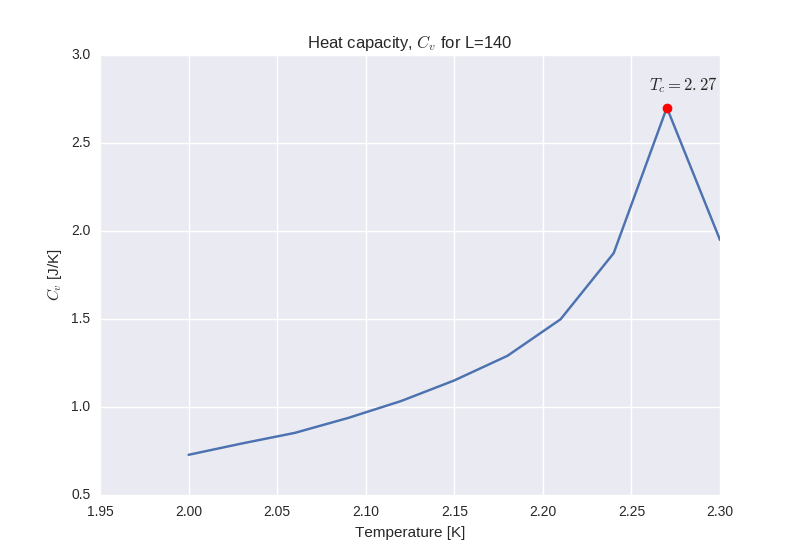
\includegraphics[height=2.2in]{cvl140.png}
        \caption{Heat capacity for $L=140$}
    \end{subfigure}
      \caption{Development of the heat capacity for systems of different sizes, as a function of temperature. We simulated $10^5$ Monte Carlo cycles, excluding an equilibration time of 5000 cycles.}
\end{figure}
\begin{figure}[!ht]
    \centering
    \begin{subfigure}[H!]{0.5\textwidth}
        \centering
        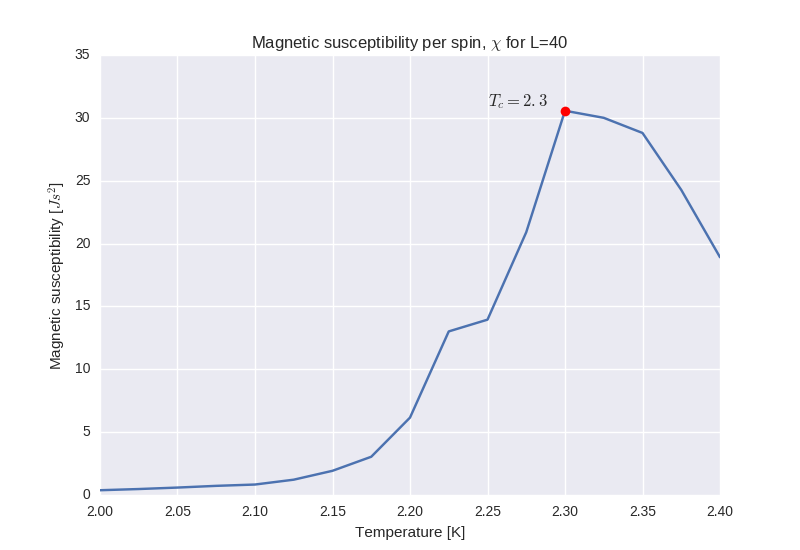
\includegraphics[height=2.2in]{chil40Ne5New.png}
        \caption{Magnetic susceptibility for $L=40$}
    \end{subfigure}%
    ~ 
    \begin{subfigure}[H!]{0.5\textwidth}
        \centering
        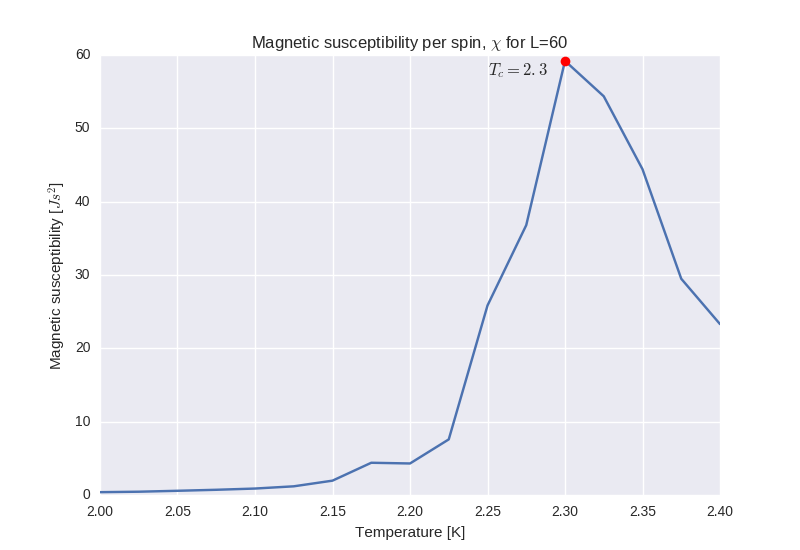
\includegraphics[height=2.2in]{chil60Ne5New.png}
        \caption{Magnetic susceptibility for $L=60$}
    \end{subfigure}
        ~
     \begin{subfigure}[H!]{0.5\textwidth}
        \centering
        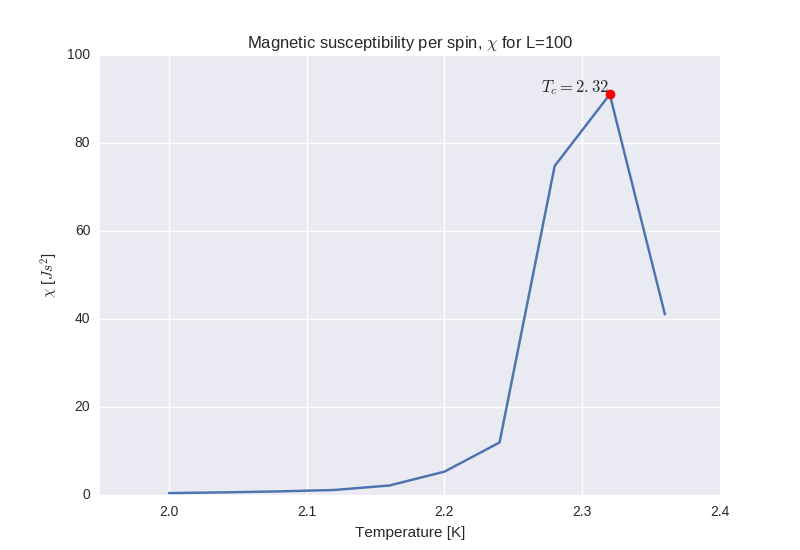
\includegraphics[height=2.2in]{chil100Ne5New.png}
        \caption{Magnetic susceptibility for $L=100$}
    \end{subfigure}%
    ~ 
    \begin{subfigure}[H!]{0.5\textwidth}
        \centering
        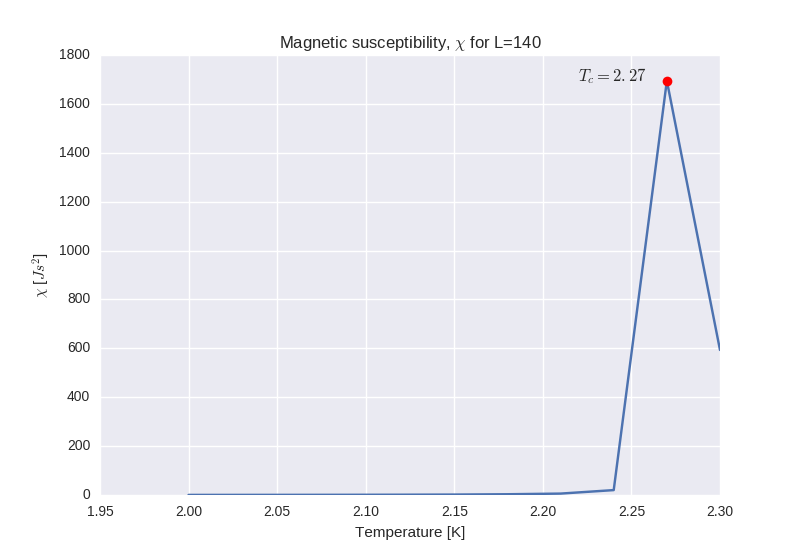
\includegraphics[height=2.2in]{chil140.png}
        \caption{Magnetic susceptibility for $L=140$}
    \end{subfigure}
      \caption{Development of the magnetic susceptibility for systems of different sizes, as a function of temperature. We simulated $10^5$ Monte Carlo cycles, excluding an equilibration time of 5000 cycles.}
\end{figure}
\subsection{Results from parallelizing our code}
\begin{table}
\centering
\caption{Comparison of speed with and without parallelization for a $20 \times 20$ lattice. We compare for numbers of Monte-Carlo cycles, $N$.}
\begin{tabular}{|c|c|c|}
\hline
N & With MPI [s] &  Without MPI [s]\\
\hline
\rule{0pt}{2ex}    
$4\cdot 10^5$ & 4.08 & 11.296 \\
$4 \cdot 10^6$ & 45.347 & 109.675\\ 
\hline
\end{tabular}
\end{table}
\section{Discussion}
\subsection{The 2 $\times$ 2 lattice}
Figure \ref{fig:2x2_nsteps} compares the analytic and numeric solution for a different number of Monte Carlo cycles. As expected, our numeric solution approaches the analytic solution with increasing $N$, and for $N=4\times 10^7$, the solutions are barely distinguishable. Therefore, we adapt this as an acceptable $N$, for this system.  Note further that, with this $N$,all other thermodynamic quantities shown in figure \ref{fig:2x2_thermo} are also very well reproduced by our code. This shows that our simulations converge to the expected values for the $2\times2$ lattice, which hopefully implies that our code also works for larger lattices, for which there are no analytic solutions. Note, however, that $N=10^7$ was not attainable within our strict time constraints. Therefore, we performed the remaining simulations with $N=10^5$, but start the computation after equilibrium has  been reached. Note that this means the system does not have to "balance out" the large errors in 
\section{Conclusion}
\end{document}